
% sezione intro frame 01
\begin{frame}
    \frametitle{Introduzione al Corso di Codifica di Testi}
    \framesubtitle{Obiettivi, competenze e conoscenze}
    \addtocounter{nframe}{1}
    
    \begin{block}{Obiettivo}
        Illustrare i principi di modellazione e le prassi di codifica del testo per una adeguata rappresentazione ed elaborazione digitale di risorse testuali.  
    \end{block}

    \begin{block}{Rationale}
       Fornire gli strumenti e le conoscenze necessarie per progettare e realizzare criticamente una codifica digitale di testi complessi, in particolare testi letterari e di interesse storico-culturale, usando le linee guida della Text Encoding Initiative (TEI).
    \end{block}

\end{frame}

% sezione intro frame 02
\begin{frame}
    \frametitle{Argomenti trattati}
    \framesubtitle{Obiettivi, competenze e conoscenze}
    \addtocounter{nframe}{1}
    
    \begin{block}{Cosa ci aspettiamo alla fine del corso}
        \begin{itemize}
        \item valutare il metodo di codifica più appropriato allo scenario d'interesse
        \item creare uno schema di codifica TEI
        \item usare gli strumenti più idonei per la codifica di una risorsa testuale
        \item elaborare e visualizzare il testo codificato
        \end{itemize}
    \end{block}

\end{frame}

% sezione intro frame 03
\begin{frame}
    \frametitle{Principali Argomenti}
    \framesubtitle{Obiettivi, competenze e conoscenze}
    \addtocounter{nframe}{1}

    
        \begin{itemize}
            \item Codifica dei caratteri e di testi
            \item I linguaggi di markup e introduzione a XML
            \item Creazione di schemi di codifica
            \item Le norme TEI (Text Encoding Initiative)
            \item Alcuni specifici Moduli TEI
            \item Definizione di schemi di codifica personalizzati
            \item Introduzione ai fogli di stile XSLT
            \item Elaborazione documenti XML-TEI (XSLT2.0, DOM)
            \item Esempi, esercitazioni e seminari 
        \end{itemize}

\end{frame}

\begin{frame}
    \frametitle{Bozza piano del Corso: Calendario 2018/2019}
    \framesubtitle{Lunedì dalle 14.00 alle 18.00}
    \addtocounter{nframe}{1}
    
        \begin{itemize}
            \setlength\itemsep{0.5em}
            \item Lezione 1 (24/9): Introduzione al corso e strumenti software utilizzati
            \item Lezione 2 (1/10): Elementi teorici relativi alla rappresentazione del testo
            \item Lezione 3 (8/10) Elementi di XML e introduzione alla definizione degli Schemi XML
            \item Lezione 4 (15/10): Elementi di Codifica TEI
            \item Lezione 5 (22/10): Modulo Specifico TEI
        \end{itemize}

\end{frame}

\begin{frame}
    \frametitle{Bozza piano del Corso: Calendario 2018/2019}
    \framesubtitle{Lunedì dalle 14.00 alle 18.00}
    \addtocounter{nframe}{1}
    
        \begin{itemize}
            \setlength\itemsep{0.5em}
            \item Lezione 6 (29/10): Moduli Editoriali TEI
            \item Lezione 7 (5/11): Codifica dei caratteri e Unicode
            \item Lezione 8 (12/11): Elaborazione documenti XML-TEI (XSLT e DOM)
            \item Lezione 9 (19/11): Esercitazione e discussione sui progetti 
            \item Lezione 10 (26/11): Esercitazione e Recupero Argomenti
            \item (03/12-17/12):  Eventuali esercitazioni, attività laboratoriali, recupero argomenti
        \end{itemize}

\end{frame}

% sezione intro frame 04
\begin{frame}
    \frametitle{Perché è importante la codifica dei testi}
    \framesubtitle{Motivazioni pratiche}
    \addtocounter{nframe}{1}
    
    \begin{block}{Dove troviamo i testi}
        Nella nostra cultura tradizionale la quasi totalità dei testi è ``registrata'', ``trasmessa'' e quindi ``conservata'' attraverso supporti e materiali fisici di varia natura e forma (iscrizioni su pietra, manoscritti di pergamena, papiri, carta, libri a stampa, incunabula, cinquecentine, etc).
    \end{block}

\end{frame}

% sezione intro frame 04b
\begin{frame}
    \frametitle{Perché è importante la codifica dei testi}
    \framesubtitle{Dove troviamo i testi}
    \addtocounter{nframe}{1}
    
    \begin{center}

        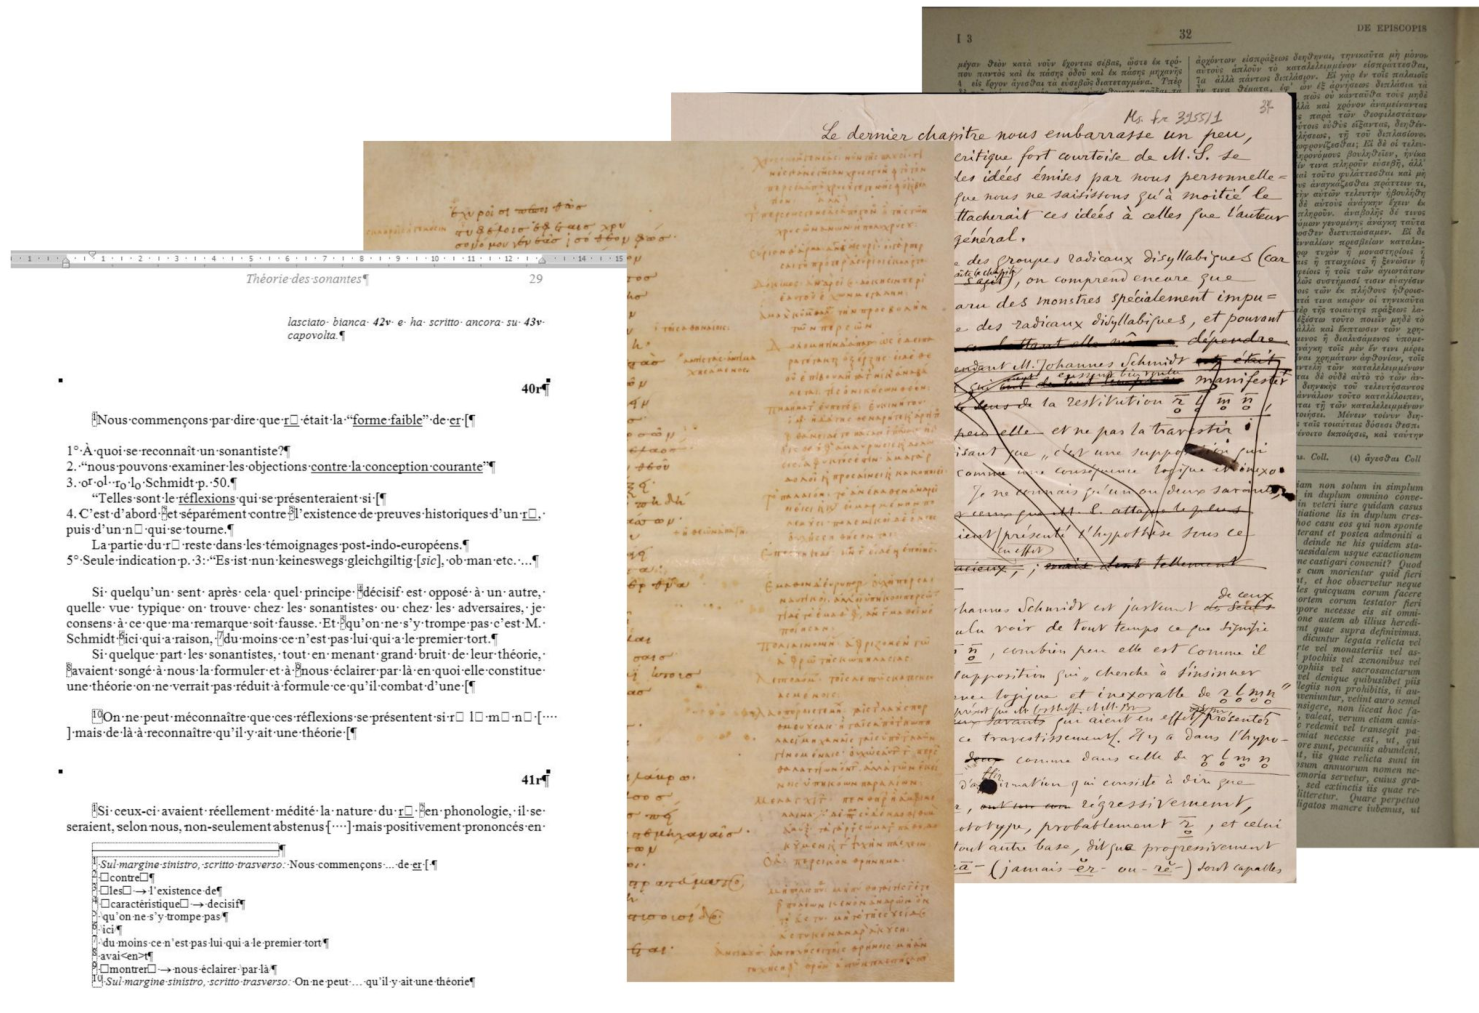
\includegraphics[width=.9\textwidth]{imgs/TestiVariSupporti.pdf}

    \end{center}

\end{frame}

\begin{frame}
    \frametitle{Perché è importante la codifica dei testi}
    \framesubtitle{Dove troviamo i testi}
    \addtocounter{nframe}{1}
    
    \begin{center}

        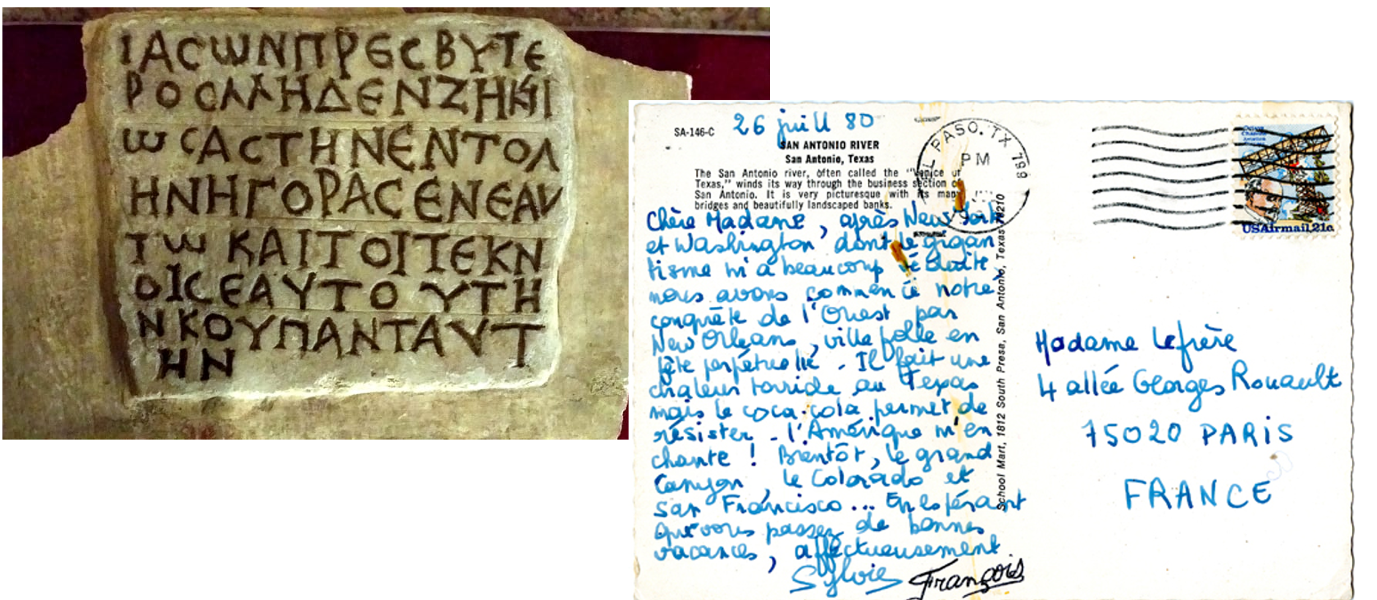
\includegraphics[width=.9\textwidth]{imgs/postCardStone.png}

    \end{center}

\end{frame}

% sezione intro frame 05
\begin{frame}
    \frametitle{Perché è importante la codifica dei testi}
    \framesubtitle{Motivazioni pratiche}
    \addtocounter{nframe}{1}
    
    \begin{block}{Perché codificare i testi}
        Per rendere disponibile questo patrimonio attraverso i sistemi per la gestione dell'informazione digitali e computazionali è necessario effettuare una trasposizione/transcodifica\textsuperscript{*} dei testi dal loro supporto originario verso il nuovo supporto elettronico (\textit{Machine Readable Form}).
    \end{block}

    \begin{center}
        * \textit{procedimento di conversione dei dati codificati secondo un sistema verso un sistema diverso}
    \end{center}

\end{frame}

% sezione intro frame 06
\begin{frame}
    \frametitle{Perché è importante la codifica dei testi}
    \framesubtitle{Motivazioni teoriche}
    \addtocounter{nframe}{1}
    
    \begin{block}{Scienze umane vs Scienze informatiche}
        Il rapporto tra sapere umanistico e informatica non è solo una questione meramente strumentale:\\ 
        \textit{l'informatica non è solo un utensile dalle notevoli capacità.}

        \begin{center}
            Salto di paradigma sia da un punto di vista teorico sia metodologico.
        \end{center} 
    \end{block}

\end{frame}

%sezione intro frame 06b
\begin{frame}
    \frametitle{Perché è importante la codifica dei testi}
    \framesubtitle{Motivazioni teoriche}
    \addtocounter{nframe}{1}
    
    \begin{block}{La codifica come metodologia}
        L'attività di codifica diviene metodo di analisi della conoscenza nell'ambito delle discipline che si occupano del testo.
     \end{block}

     \begin{block}{La codifica come analisi teorica}
     Il linguaggio di codifica adottato può essere considerato come un linguaggio teorico:
      
     \begin{center}
        \textit{Esplicitare e formalizzare le ipotesi interpretative su un certo oggetto di studio}
     \end{center} 
    \end{block}

\end{frame}

% sezione intro frame 07
\begin{frame}
    \frametitle{Perché è importante la codifica dei testi}
    \framesubtitle{In sintesi}
    \addtocounter{nframe}{1}
    
    \begin{block}{Rappresentare il testo}
         Il focus del corso sarà incentrato sulla rappresentazione digitale del testo.
    \end{block}

    \begin{block}{Esistono dibattiti e controversie}
        Per ottenere una rappresentazione digitale del testo ci sono diversi formati, formalismi e prassi:
        \\ la nostra scelta ricade sulle norme suggerite dal consorzio TEI.
    
        Molte questioni non sono risolte altre sono controverse, sia dal punto di vista teorico-metodologico, sia pratico-tecnologico.
   
    \end{block}

\end{frame}

% sezione intro frame 08
\begin{frame}
    \frametitle{Perché è importante la codifica dei testi}
    \framesubtitle{Ma in definitiva}
    \addtocounter{nframe}{1}
    
    \begin{block}{Perché codificare}

        \begin{center}
            \textit{Le differenze di formato sono più che altro estetiche e non sostanziali}
        \end{center}

    \end{block}
     

    \begin{block}{Perché codificare}

        \begin{center}
            \textbf{Ma anche l'occhio \underline{umano} vuole la sua parte}
        \end{center}
       
    \end{block}

\end{frame}

% Lo studio del sapere ha come oggetto immediato i testi (letterari e non). Nella nostra cultura la quasi totalità dei testi letterari (fino a questo momento) è costituita da testi scritti su supporti cartacei di varia natura e forma.